% This file includes the formatting guidelines for papers submitted to 'Inteligencia Artificial' (Revista Iberoamericana de IA)
% It should be used jointly with file iberamia.sty

\documentclass[10pt,a4paper,twoside]{article}
\usepackage[english]{babel}
\usepackage[latin1]{inputenc}
\usepackage{amssymb}
\usepackage{amsmath}
\usepackage{fancyhdr}
%\usepackage[usenames,dvips]{color}
\usepackage{verbatim}
\usepackage{lastpage}
\usepackage{ifthen}
\usepackage{csquotes}
\usepackage{cite}

\newcommand{\norm}[1]{\left\lVert#1\right\rVert}
\DeclareMathOperator*{\argmin}{arg\,min}
\DeclareMathOperator*{\argmax}{arg\,max}


%%%%%%%%%%%%%%%%%%%%%%%%%%%%%%%%%%%%%%%%%%
%                                        %
% IMPORTANT FOR USERS OF PDFLATEX        %
%                                        %
%%%%%%%%%%%%%%%%%%%%%%%%%%%%%%%%%%%%%%%%%%
%
% We assume LaTeX users will use PDFLaTeX
% Comment the next lines if you wish to use dvipdfm instead.
\usepackage[pdftex]{color,graphicx}
\usepackage{hyperref}
%
% Remove comment if you wish to use dvipdfm to generate PDF files.
%\usepackage{epsfig}
%\usepackage[dvipdfm]{hyperref}
%
%%%%%%%%%%%%%%%%%%%%%%%%%%%%%%%%%%%%%%%%%%

\usepackage{iberamia}   %Journal's style file iberamia.sty

%Publication data:
\newcommand{\thispaperdoi}{}
\setcounter{year}{2017}
\setcounter{volume}{20}
\setcounter{issue}{59}
\setcounter{page}{123}


\title{From Imitation to Prediction, Data Compression vs Recurrent Neural Networks for Natural Language Processing}

%%NOTE: If you are submitting for review, do not include author's data
%       The journal uses a double-blind review processe

\author{Juan Andr�s Laura, Gabriel Omar Masi, Luis Argerich
\smallskip \\
\small{Departemento de Computaci�n,
	Facultad de Ingenier�a. Universidad de Buenos Aires\\
please@do.not.include.email
\smallskip \\
jandreslaura@gmail.com, masigabriel@gmail.com, largerich@fi.uba.ar 
}}
\date{}

\begin{document}

\medskip
\maketitle

\pagestyle{Rest}
\thispagestyle{FirstPage}
\smallskip


\noindent{\small{{\textbf Abstract}
In recent studies \cite{Graves}\cite{Sutskever}\cite{Bown} Recurrent Neural Networks were used for generative processes and their surprising performance can be explained by their ability to create good predictions. In addition, data compression is also based on prediction. What the problem comes down to is whether a data compressor could be used to perform as well as recurrent neural networks in the natural language processing tasks of sentiment analysis and automatic text generation. If this is possible, then the problem comes down to determining if a compression algorithm is even more intelligent than a neural network in such tasks. In our journey, a fundamental difference between a Data Compression Algorithm and a Recurrent Neural Network has been discovered. }}


\medskip

\noindent{\small{\textbf{Keywords}: KeyWord1, Keyword2, KeyWord3.}}


\section{Introduction}
One of the most interesting goals of Artificial Intelligence is the simulation of different human creative processes like speech recognition, sentiment analysis, image recognition, automatic text generation, etc. In order to achieve such goals, a program should be able to create a model that reflects how humans think about these problems.

Researchers think that Recurrent Neural Networks (RNN) are capable of understanding the way some tasks are done such as music composition, writing of texts, etc. Moreover, RNNs can be trained for sequence generation by processing real data sequences one step at a time and predicting what comes next\cite{Graves}\cite{Sutskever}.

Compression algorithms are also capable of understanding and representing different sequences and that is why the compression of a string could be achieved. However, a compression algorithm might be used not only to compress a string but also to do non-conventional tasks in the same way as neural nets (e.g. a compression algorithm could be used for clustering\cite{Cilibrasi}, sequence generation or music composition).

Both neural networks and data compressors should be able to learn from the input data to do the tasks for which they are designed. In this way, someone could argue that a data compressor can be used to generate sequences or a neural network can be used to compress data. In consequence, using the best data compressor to generate sequences should produce better results than the ones obtained by a neural network but if this is not true then the neural network should compress better than the state of the art in data compression.

The hypothesis for this research is that, if compression is based on learning from the input data set, then the best compressor for a given data set should be able to compete with other algorithms in natural language processing tasks. In the present work, this hypothesis will be analyzed for two given scenarios: sentiment analysis and automatic text generation.

\section{Data Compression as an Artificial Intelligence Field}

For many authors there is a very strong relationship between Data Compression and Artificial Intelligence\cite{Franz}\cite{Ofir}. Data Compression is about making good predictions \cite{Ratsaby} which is also the goal of Machine Learning, a field of Artificial Intelligence. 

Essentially, Data compression involves two important steps: modeling and coding. Coding is a solved problem using arithmetic compression. The difficult task is modeling because it comes down to building a description of the data using the most compact representation; this is again directly related to Artificial Intelligence. Using the Minimal Description Length principle\cite{Grunwald} the efficiency of a good Machine Learning algorithm can be measured in terms of how good it is to compress the training data plus the size of the model itself.

A file containing the digits of $\pi$ can be compressed with a very short program able to generate those digits, gigabytes of information can be compressed into a few thousand bytes. However, the problem arises when trying to find a program capable of understanding that our input file contains the digits of $\pi$. In consequence, achieving the best compression rate involves finding a program able to always find the most compact model to represent the data and that is clearly an indication of intelligence, perhaps even of General Artificial Intelligence. 

\section{RNNs for Data Compression}

Recurrent Neural Networks and in particular LSTMs were used not only for predictive tasks\cite{Gers} but also for Data Compression\cite{Schmidhuber}. While the LSTMs were brilliant in their text\cite{Sutskever}, music\cite{Bown} and image generation\cite{Gregor} tasks, they were never able to defeat the state of the art algorithms in Data Compression\cite{Schmidhuber}. 

This might indicate that there is a fundamental difference between Data Compression and Generative Processes and between Data Compression Algorithms and Recurrent Neural Networs. After experiments, a fundamental difference will be shown in this research in order to explain why a RNN can be the state of the art in some generatives process but not in Data Compression.

\section{Sentiment Analysis}

\subsection{A Qualitative Approach}

Human feelings can be determined according to what they write in many social networks such as Facebook, Twitter, etc.. It looks like an easy task for humans. However, it could be not so easy for a computer to automatically determine the sentiment behind a piece of writing.

The task of guessing the sentiment of text using a computer is known as Sentiment Analysis and one of the most popular approaches for this task is to use neural networks. In fact, Stanford University created a powerful neural network for sentiment analysis\cite{Socher} which is used to predict the sentiment of movie reviews taking into account not only the words in isolation but also the order in which they appear. In the first experiment, the Stanford neural network and a PAQ compressor\footnote{PAQ's source code is free and it is available at Mahoney's web \cite{Mahoney}}\cite{Mahoney} will be used for doing sentiment analysis of movie reviews in order to determine whether a user likes or not a given movie (i.e. each movie review will be classified as positive or negative). After that, results obtained will be compared using the percentage of correctly classified movie reviews. Both algorithms will use a public data set for movie reviews\cite{Maas}.

In order to understand how sentiment analysis could be done with a data compressor it is important to comprehend the concept of using Data Compression to compute the distance between two strings using the \textit{Normalized Compression Distance}\cite{Vitanyi}.

$$
NCD(x,y) = \frac{C(xy)-\min\{C(x),C(y)\}}{\max\{C(x),C(y)\}}
$$

Where $C(x)$ is the size of applying the best possible compressor to $x$ and $C(xy)$ is the size of applying the best possible compressor to the concatenation of $x$ and $y$. 

The NCD is an approximation to the Kolmogorov distance between two strings using a Compression Algorithm to approximate the complexity of a string because the Kolmogorov Complexity is uncomputable. 

The principle behind the NCD is quite simple: when string $y$ is concatenated after string $x$ then $y$ should be highly compressed whenever $y$ is very similar to $x$ because the information in $x$ contains everything needed to describe $y$. An observation is that $C(xx)$ should be equal, with minimal overhead difference to $C(x)$ because Kolmogorov complexity of a string concatenated to itself is equal to the Kolmogorov complexity of the string. 

As introduced, a data compressor performs well when it is capable of understanding the data set that will be compressed. This understanding often grows when the data set becomes bigger and in consequence compression rate improves. However, it is not true when future data (i.e. data that has not been compressed yet) has no relation with already compressed data because the more similar the information it is the better compression rate is achieved. 

Let $C(X_1,X_2...X_n)$ be a compression algorithm that compresses a set of n files denoted by $X_1,X_2...X_n$. Let $P_1,P_2...P_n$ and $N_1,N_2...N_m$ be a set of $n$ positive reviews and $m$ negative reviews respectively. Then, a review $R$ can be predicted positive or negative using the following inequality:

$$C(P_1,...P_n,R)-C(P_1,...,P_n) < C(N_1,...,N_m,R)-C(N_1,...,N_m)$$

The formula is a direct derivation from the NCD. When the inequality is not true, a review is predicted negative. 

The order in which files are compressed must be considered. As you could see from the proposed formula, the review $R$ is compressed last. 

Some people may ask why this inequality works to predict whether a review is positive or negative. So it is important to understand this inequality. Suppose that the review $R$ is a positive one. $R$ will be compressed in order to classify it: if $R$ is compressed after a set of positive reviews then the compression rate should be better than the one obtained if $R$ is compressed after a set of negative reviews because the review $R$ has more related information with the set of positive reviews and in consequence should be compressed better. Interestingly, both the positive and negative set could have different sizes and that is why it is important to subtract the compressed file size of both sets in the inequality.

\subsection{Data Set Preparation}

The Large Movie Review Dataset\cite{Maas}, which has been used for Sentiment Analysis competitions, is used in this research\footnote{Both training set and test set were chosen randomly}.


\begin{table}[hb]
	\begin{center}
		{\caption{Movie review dataset.}\label{tab:sample}}
		\begin{tabular}{|l|l|l|}
			\hline
			& Positive & Negative\\
			\hline
			Total & 12491 & 12499\\
			\hline
			Training & 9999 & 9999\\
			\hline
			Test & 2492 & 2500\\
			\hline
		\end{tabular}
	\end{center}
\end{table}

\subsection{PAQ for Sentiment Analysis}

Using Data Compression for Sentiment Analysis is not a new idea. It has been already proposed in IEEE 12th International Conference\cite{Ziegelmayer}. However, the authors did not use PAQ compressor.

PAQ Compressor is taken into account for this research because of its excellent compression rates achieved at Hutter's Prize\cite{Hutter} and many benchmarks such as Matt Mahoney's one\cite{Mahoney}.

In order to make sentiment analysis of a movie review using PAQ, it is needed to compress each review after compressing both the positive train set and the negative one separately. Given the fact that compressing each train set takes a considerable time, a checkpoint tool is used in this work. The review is classified positive if the compression rate using the positive train set is better than the one obtained using the negative train set. Otherwise, it is classified as negative. If both compression rates are equals, it is classified as inconclusive.

\subsection{Experiment Results}

In this section, the results obtained are explained by giving a comparison between the data compressor and the Stanford?s Neural Network for Sentiment Analysis. 

The following table shows the results obtained


\begin{table}[hb]
	\begin{center}
		{\caption{PAQ vs RNN Classification Results.}\label{tab:sample}}
		\begin{tabular}{|l|l|l|l|}\hline
			&\textbf{Correct}&\textbf{Incorrect}&\textbf{Inconcluse} \\ \hline
			PAQ & 77.20\% & 18.41\% & 	4.39\% \\ \hline
			RNN & 70.93\% & 23.60\% & 5.47\% \\ \hline
		\end{tabular}
	\end{center}
\end{table}

As you could see from the previous table, 77.20\% of movie reviews were correctly classified by the PAQ Compressor whereas 70.93\% were well classified by the Stanford?s Neural Network. 

There are two main points to highlight according to the result obtained:
\begin{enumerate}
	\item Sentiment Analysis could be achieved with a PAQ compression algorithm with high accuracy ratio.
	\item In this particular case, a higher precision can be achieved using PAQ rather than the Stanford Neural Network for Sentiment Analysis.
\end{enumerate}

We observed that PAQ was very accurate to determine whether a review was positive or negative, the missclassifications were always difficult reviews and in some particular cases the compressor outdid the human label, for example consider the following review:
\newline
\begin{displayquote}
	\textit{``The piano part was so simple it could have been picked out with one hand while the player whacked away at the gong with the other. This is one of the most bewilderedly trance�state inducing bad movies of the year so far for me.''}
	\newline
\end{displayquote}
This review was labeled positive but PAQ correctly predicted it as negative, since the review is misslabeled it counted as a miss in the automated test.

Analyzers based on words like the Stanford Analyzer tend to have difficulties when the review contains a lot of uncommon words. However, they can work well in longer documents by relying on a few words with strong sentiment like 'awesome' or 'exhilarating'\cite{Socher}. It was surprising to find that PAQ was able to correctly predict those.
Consider the following review:
\newline

\begin{displayquote}
	\textit{``The author sets out on a ``journey of discovery'' of his ``roots'' in the southern tobacco industry because he believes that the (completely and deservedly forgotten) movie ``Bright Leaf'' is about an ancestor of his. Its not, and he in fact discovers nothing of even mild interest in this absolutely silly and self-indulgent glorified home movie, suitable for screening at (the director's) drunken family reunions but certainly not for commercial - or even non-commercial release. A good reminder of why most independent films are not picked up by major studios - because they are boring, irrelevant and of no interest to anyone but the director and his/her immediate circles. Avoid at all costs!''}
	\newline
\end{displayquote}

This was classified as positive by the Stanford Analyzer, probably because of words such as "interest, suitable, family, commercial, good, picked", the Compressor however was able to read the real sentiment of the review and predicted a negative label. In cases like this the Compressor shows the ability to truly understand data.

\section{Automatic Text Generation}

This module?s goal is to automatically generate text with a PAQ series compressor and compare it with Andrej Karpathy RNN?s results \cite{Karpathy}, using specifics metrics and scenarios.

The ability of good compressors when making predictions is more than evident. It just requires an entry text (training set) to be compressed. At compression time, the future symbols will get a probability of occurrence: The higher the probability, the better compression rate for success cases of that prediction, on the contrary, each failure case will take a penalty. At the end of this process, a probability distribution will be associated with that input data \cite{Mahoney4}. As a result of this probabilistic model, it will be possible to simulate new samples, in other words, generate text.

\subsection{Data Model}

PAQ series compressors use arithmetic coding to encode symbols assigned to a probability distribution. Each probability lies on the interval [0,1) and when it comes to binary coding, there are two possible symbols: 0 and 1. Moreover, this compressor uses contexts, a main part of compression algorithms. They are built from the previous history and can be used to make predictions, for example, the last ten symbols can be linked to compute the prediction of the eleventh. 

PAQ uses an ensamble of several different models to compute how likely a bit 1 or 0 is next. Some of these models are based on the previous $n$ characters of $m$ bits of seen text, other models use whole words as contexts, etc. 
In order to weight the prediction performed by each model, a neural network is used to determine the weight of each model \cite{Matt3}:

$$P(1|c) = \sum_{i=1}^{n} P_i(1|c) W_i$$

Where $P(1|c)$ is the probability of bit 1 with context "c", $P_i(1|c)$ is the probability of bit 1 in context "c" for model $i$ and $W_i$ is the weight assigned to model $i$.

In addition, each model adjusts their predictions based on the new information. When compressing, input text is processed bit by bit. On every bit, the compressor updates the context of each model and adjusts the weights of the neural network. 

Generally, as you compress more information, predictions improve.

\subsection{Text Generation}

When data set compression is over, PAQ is ready to generate text. A random number is sampled in the [0,1) interval and transformed into a bit 1 or 0 using Inverse Transform Sampling \cite{InverseSampling}. In other words, if the random number falls within the probability range of symbol 1, bit 1 is generated, otherwise, bit 0. 

\begin{figure}[hb]
	\begin{center}
		\includegraphics[angle=0,width=0.5\textwidth]{paq.png}
		\caption{PAQ splits the [0,1) interval giving $1/4$ of probability to bit 0 and $3/4$ of probability to bit 1. When a random number is sampled in this context it is more likely to generate a 1. Each generated bit updates all models' context. However, that bit should not be learned becaused of its random nature. In other words, PAQ just learns from the training set and then generates random text using that probabilistic model. After 8 bits, a character is generated.}
		\label{fig1}
	\end{center}
\end{figure}

\section{References}
References should be clear and complete. Sample references are these
\cite{pearl1984} \cite{hartetal1968} \cite{korf1985} and this one
\cite{oetikeretal2008}. Do not forget to include DOI numbers in your
references when available. You can associate hyperlinks to DOI numbers
in \LaTeX using the \textbackslash doi command, see for example
\cite{vovk2007}. Please, pay attention to the difference with
\cite{oetikeretal2008} that explicitly includes a URL, and not a DOI
reference. See below the format of references. \LaTeX users are
encouraged to use Bibtex.

\subsection{What is a DOI?}
The DOI (Digital Object Identifier) is a unique identifier assigned by
publishers to electronically published items (books, journal papers,
etc.) The DOI system provides a framework for persistent
identification. The physical location of a digital object may change
over time, but its DOI name will not change. Currently, a DOI number
can be resolved prefixing http://dx.doi.org/ to the DOI. Therefore
links of the form http://dx.doi.org/[DOI] are expected to work
properly over time, regardless of the physical location changes of the
referenced items. To learn more about the DOI see
\url{http://www.doi.org}

\subsection{Where can I find the DOI of my references?}
DOI numbers should appear explicitly in the first page of printed
journal papers, either at the top or bottom of the page, like in
figure \ref{fig:print-doi}. Electronic journals display DOI numbers in
the papers access or home pages, like in figure \ref{fig:home-doi}. If
you cannot find the DOI of a reference at first sight it probably does
not have one, so do not worry. Many articles do not have DOI numbers
assigned (specially older ones).

\begin{figure}
  \begin{center}
    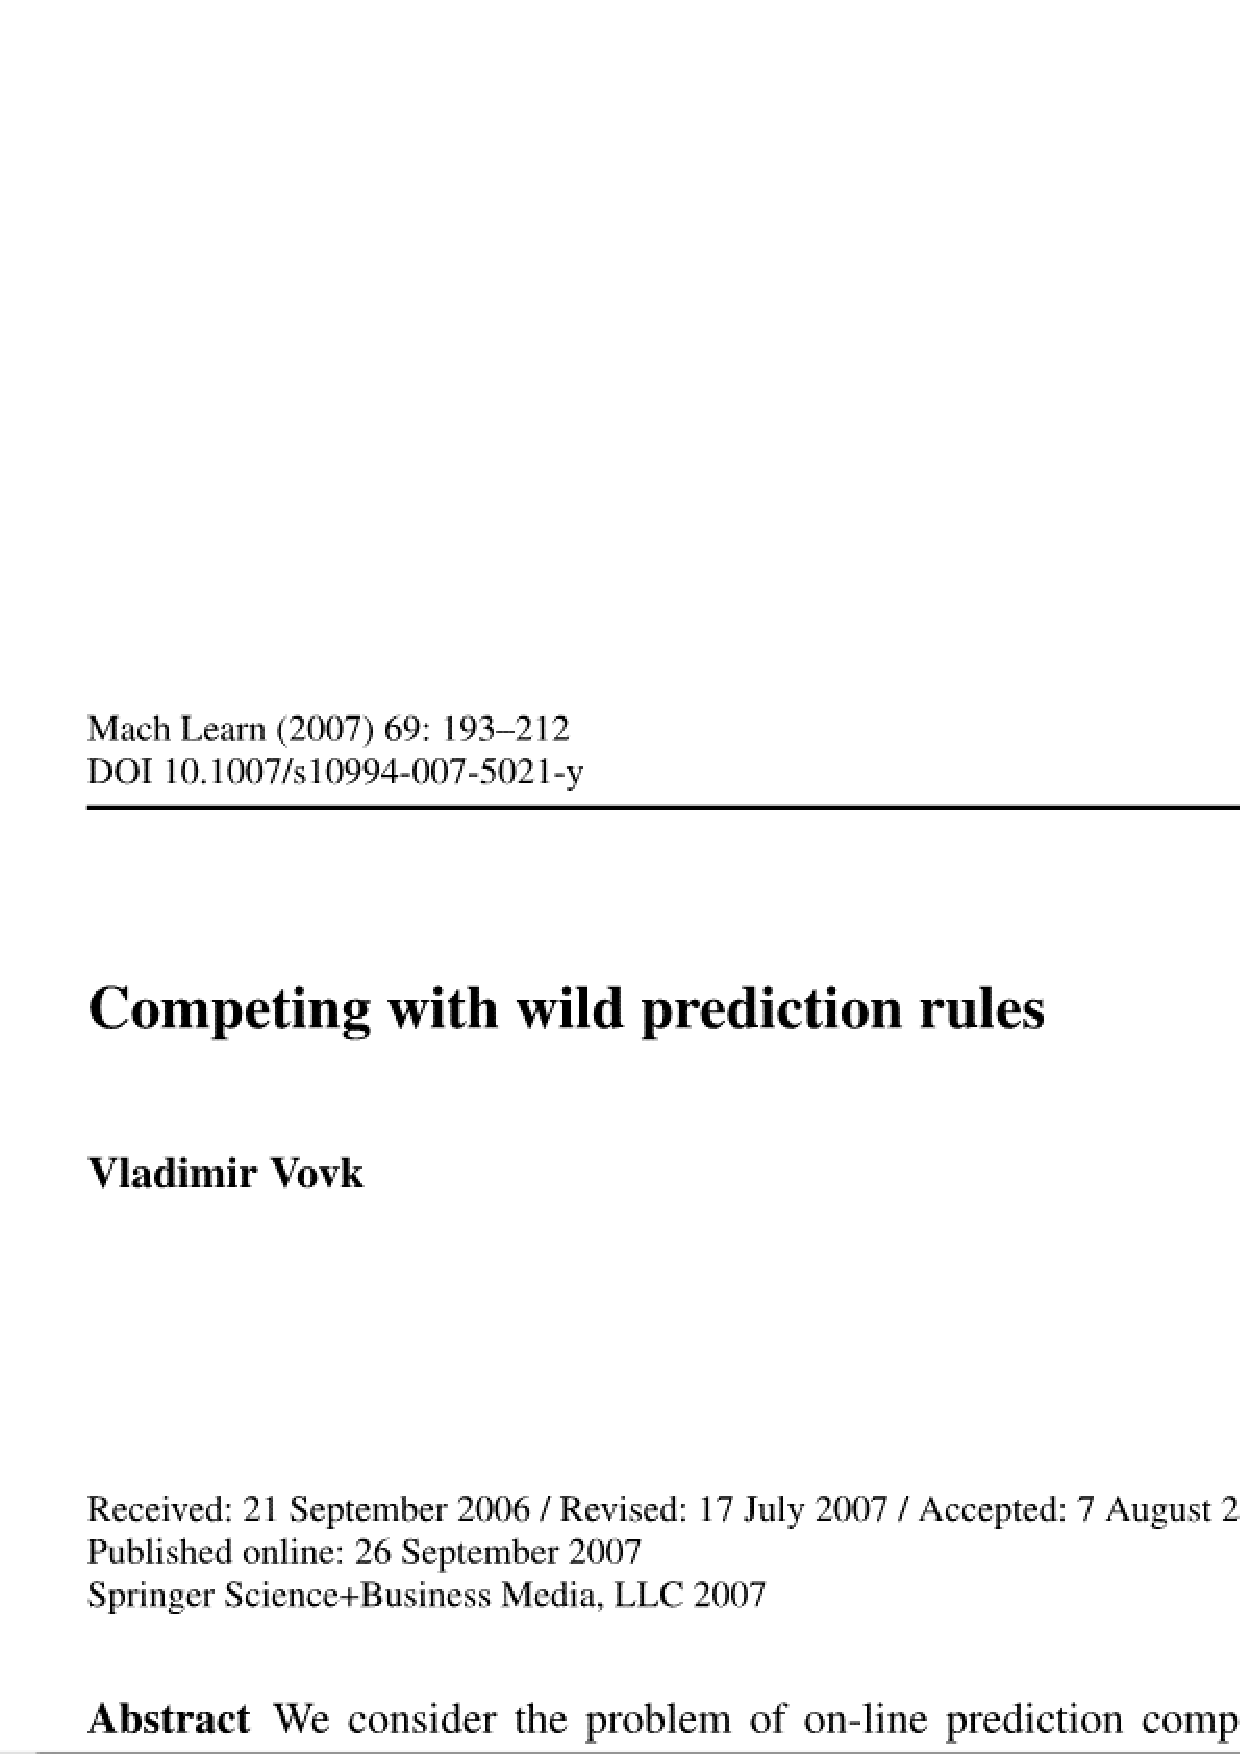
\includegraphics[angle=0,width=0.7\textwidth]{print-doi}
    \caption{DOI in a printed document.}
    \label{fig:print-doi}
 \end{center}
\end{figure}

\begin{figure}
  \begin{center}
    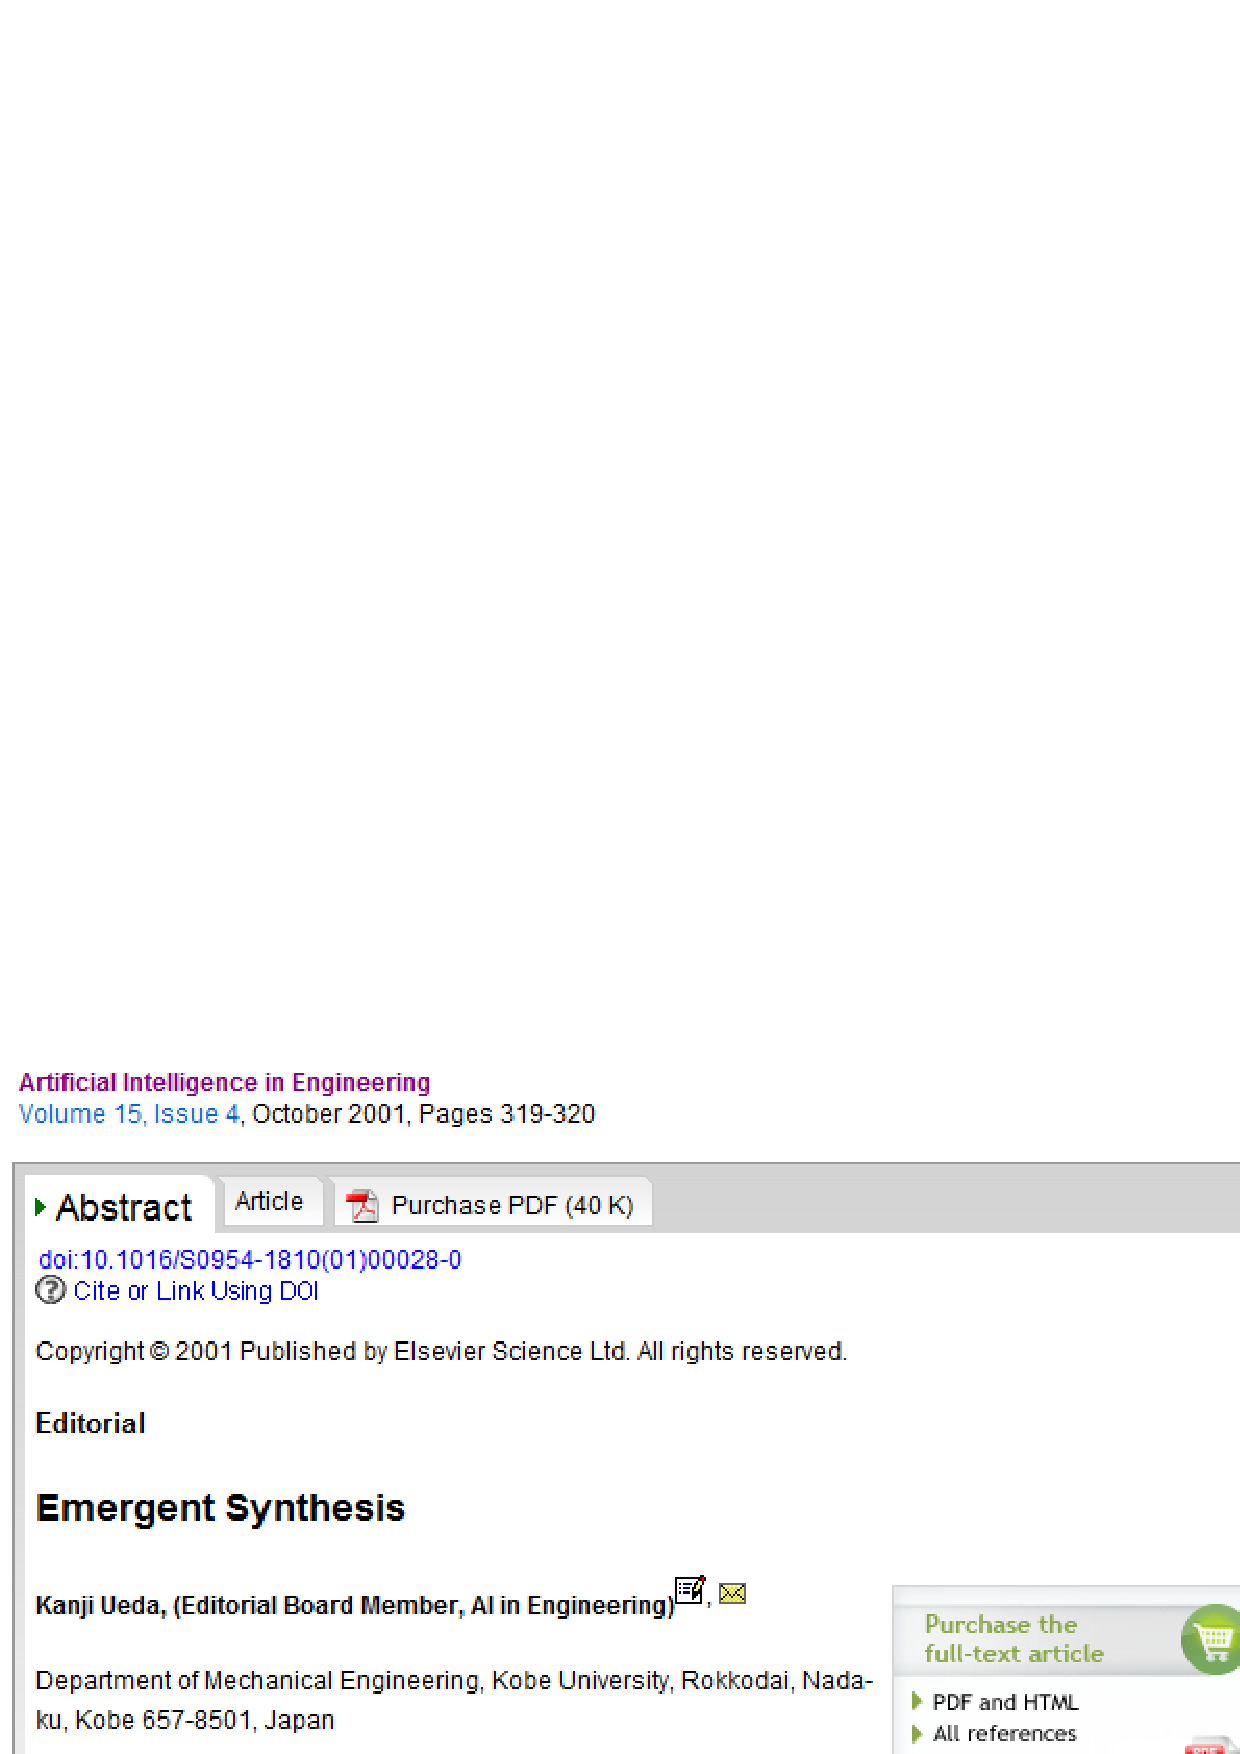
\includegraphics[angle=0,width=0.7\textwidth]{home-doi}
    \caption{DOI in a document available on the Web.}
    \label{fig:home-doi}
 \end{center}
\end{figure}

\subsection{Why is it important to include DOI numbers in references
  (when available)?}

New papers published by Inteligencia Artificial are assigned a DOI
number as a free service to their authors. Documents receiving a DOI
are expected to include DOI numbers in their own references.

Including DOI numbers in your references (when available) will make
your paper more useful and comfortable to read for readers and
reviewers. If you are a \LaTeX user and include DOI numbers as
explained above, the related hyperlinks will be added automatically to
your document.

\section{Journal Scope}
Inteligencia Artificial is a quarterly journal promoted and sponsored by Iberamia (Sociedad Iberoamericana de Inteligencia Artificial)(http://iberamia.dsic.upv.es/inicial.html). The journal publishes high-quality original research papers reporting theoretical or applied advances in all branches of Artificial Intelligence. In addition to rapid publication and dissemination of unsolicited contributions, Inteligencia Artificial is committed to producing monographs and special issues on topics of special relevance to the AI community.

\section{Manuscript Submission and Review}

Paper submission should be carried out through the journal's Web page http://journal.iberamia.org. Click the ``ABOUT'' button and follow the author's guidelines.

Following this process the author implicitly transfers copyright of
accepted papers to IBERAMIA, accepting their publication electronically
(freely available through the Journal's Web pages) and in printed
volumes.

Inteligencia Artificial welcomes research papers written in Spanish or
English. Manuscripts should be uploaded in PDF format through the
journal's Web pages (http://journal.iberamia.org - link 'Submissions').
All research papers falling within the journal's scope will be subject
to double-blind peer-review by at least two anonymous
reviewers. Authors must omit their names in submitted manuscripts. The
journal publishes four issues per year, each one at the start of each
season (spring, summer, autumn, and winter). The journal will not
carry out editing of manuscripts. Authors should adhere strictly to
the norms in the "Journal's formatting guidelines".  Accepted papers
will be published electronically at the journal's Web pages, with free
access from the Internet. The journal encourages authors to add links
in their personal pages pointing to the journal's pages containing
their contributions.

\section{Originality and Copyright}
Research papers submitted to Inteligencia Artificial cannot have been
published previously, nor be under review for publication
elsewhere. However, the journal welcomes extended and improved
versions of papers published in conferences and workshops, which will
be subject to a new peer-review process.  Authors implicitly accept
publication of submitted papers by , both electronically (with
free access from the Internet) and in print, as well as dissemination
through other media and entities with which IBERAMIA may establish
agreement, transferring IBERAMIA all the necessary rights.

\section{Monographs and Special Issues}
The journal welcomes monograph or special issue proposals related to
specific areas of Artificial Intelligence. Proposals to coordinate
monographs or special issues should be sent through email to the
Editor (editor@iberamia.org).  Contributions to monographs or special
issues can be original works including new research papers, extended
and improved versions of papers published in conferences and
workshops, and survey papers that summarize the topics of a particular
monograph or special issue. In all cases, the publication of
contributions is conditioned to acceptance in a new peer-review
process carried out by an international scientific committee under the
journal's supervision.

\section{Theses Summaries }
Inteligencia Artificial is specially interested in the publication of
Ph.D. dissertation summaries that provide a quick and state-of-the-art
reference in particular topics of Artificial Intelligence. Summaries
can be submitted following the regular submission process, stating
"RESUMEN DE TESIS" in the heading, and should be limited to 2-4 pages.


\section*{Acknowledgements}
This is the place for acknowledgements.

\bibliographystyle{plain}
\bibliography{References}         %Check the iberamia.bib file

\end{document}
